W sieciowym modelu obliczeń przyjmujemy, że każdy węzeł wyposażony jest w pamięć lokalną i wykonuje własne operacje. Węzeł może przetwarzać dane w swojej pamięci lokalnej oraz wsyłać i odbierać dane od innych węzłów sieci w postaci \emph{komunikatów}.  współdzielona przez węzły (rys. \ref{fig:model_net}) nie istnieje. Tak jak w przypadku modelu z pamięcią wspólną, operacje w sieci mogą być synchroniczne lub asynchroniczne.\\

Do każdego węzła sieci przypisany jest numer identyfikacyjny (\emph{pid}). \(\mu\)-ty węzeł oznaczamy przez \(P_\mu\). Powiemy, że \(P_\lambda\) jest \emph{sąsiadem} \(P_\mu\), jeśli istnieje bezpośrednie fizyczne połączenie między nimi.\cite{Golub}

Sposób łączenia układu jednostek obliczeniowych (procesorów) w sieć nazywamy \emph{topologią sieci}. Topologię sieci można przedstawić jako graf \(G=(N,E)\), gdzie każdy węzeł \(i\in N\) oznacza jednostkę obliczeniową, a każda krawędź \((i, j) \in E\) – dwukierunkową komunikację między jednostkami obliczeniowymi \(i\) i \(j\). 

Procesory pracujące w sieci asynchronicznej zarządzają swoimi zadaniami przez wymianę komunikatów. Schemat taki nazywamy modelem wymiany komunikatów. Procesory te niekoniecznie muszą być ze sobą sąsiadujące. 

\begin{figure}[h]
\centering
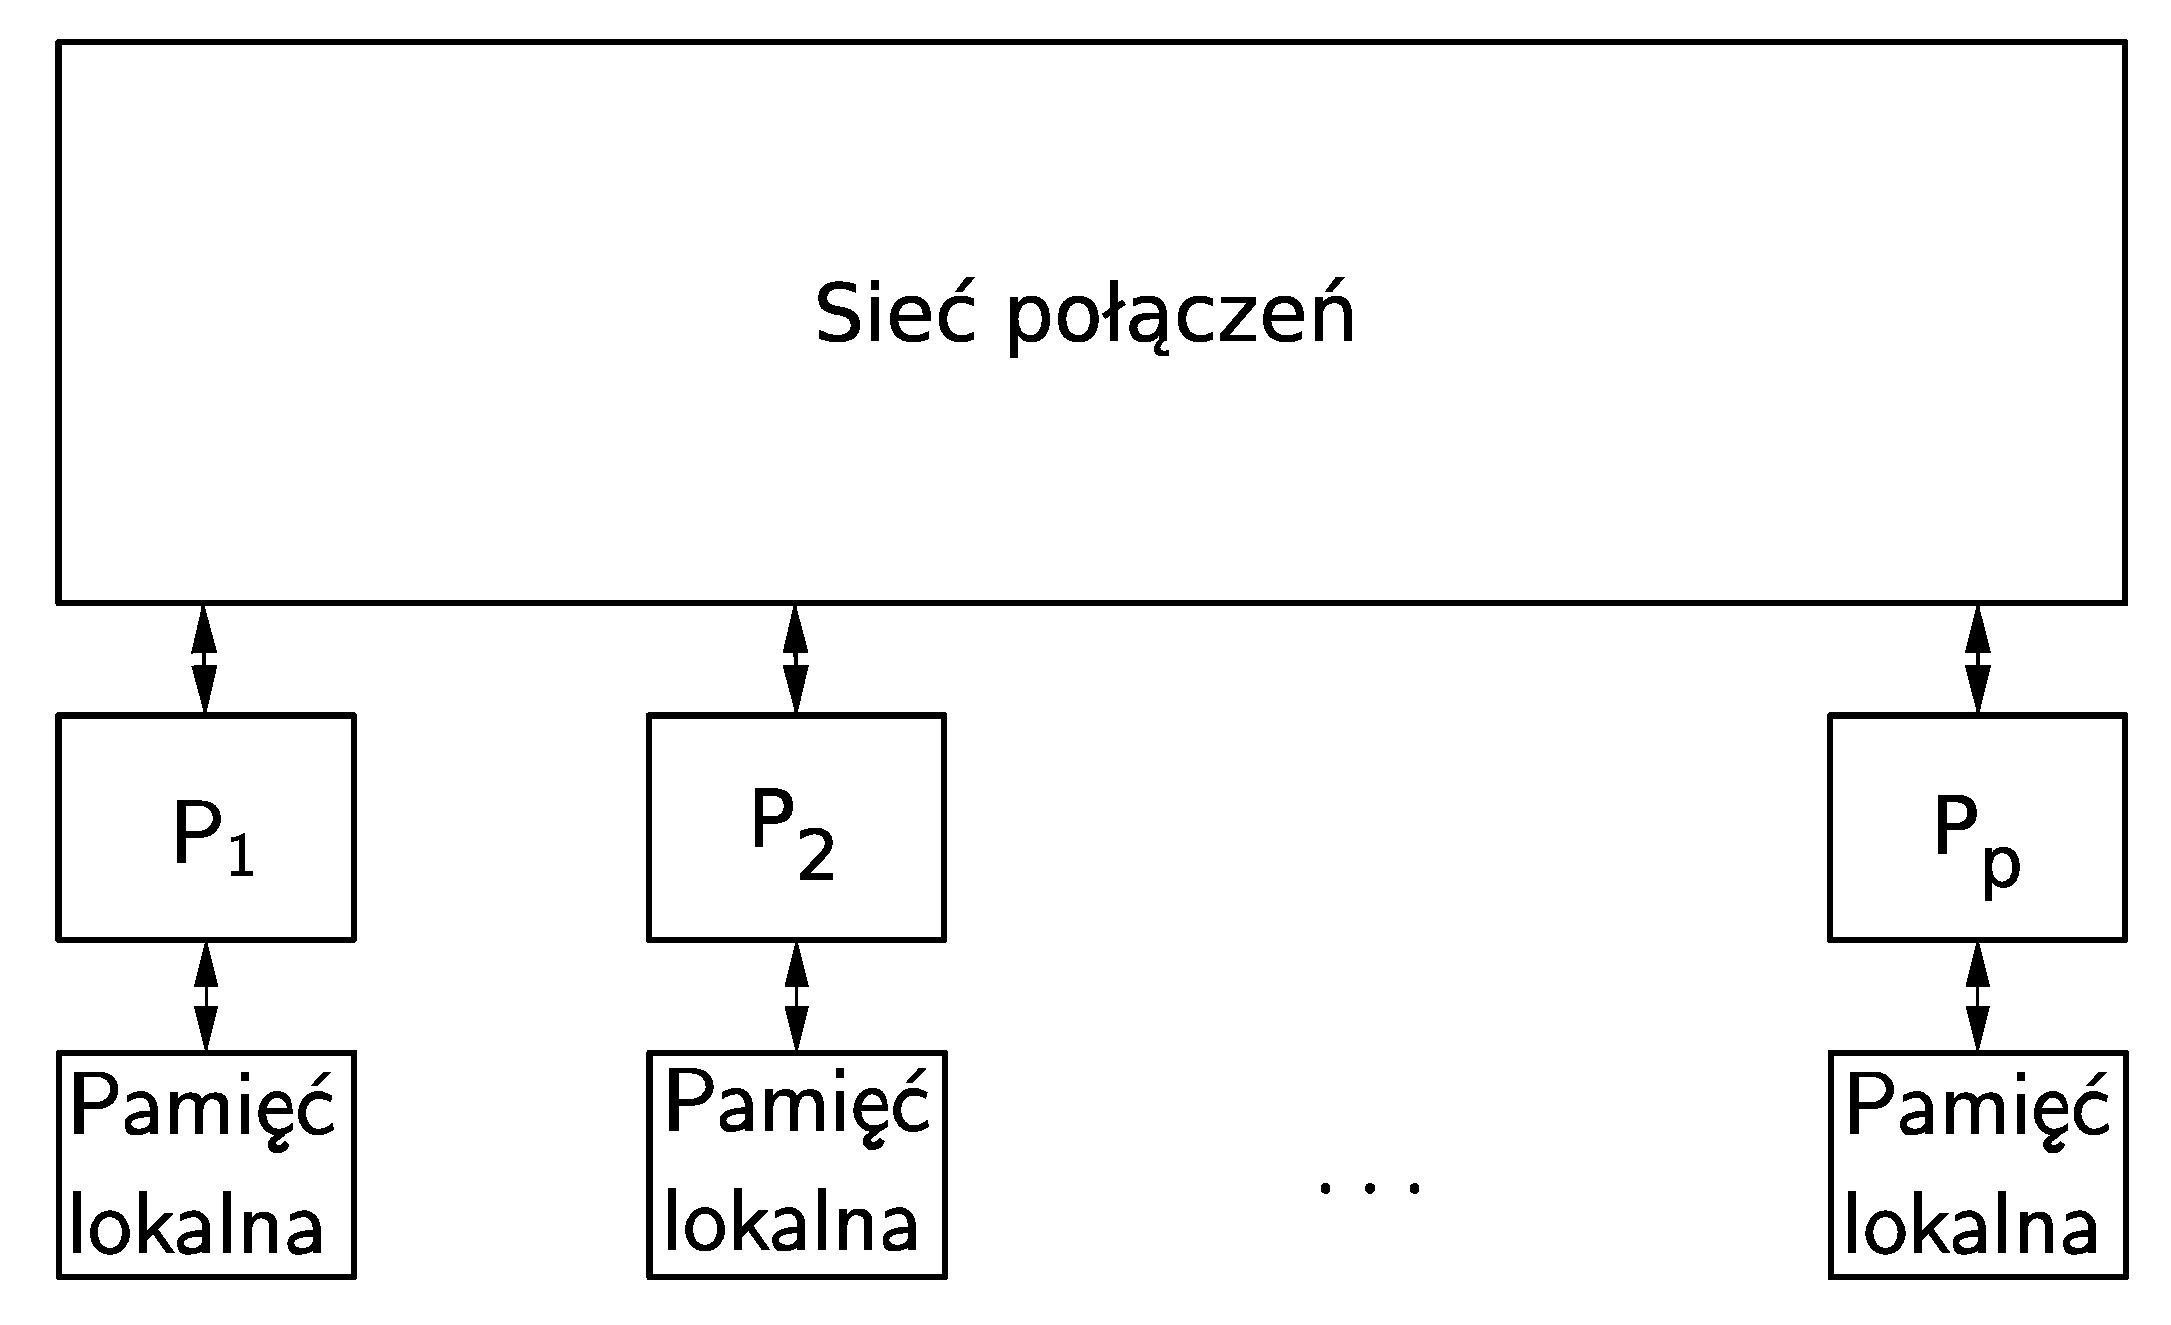
\includegraphics[width=22em]{images/Rys_net.eps}
\caption{Model sieciowy}
\label{fig:model_net}
\end{figure}

Charakteryzuje ją kilka parametrów:

\begin{enumerate}
 \item średnica – maksymalna odległość (krawędziowa) między dowolną parą węzłów; im miejsza, tym lepiej.
 \item maksymalny stopień wierzchołka – maksymalna liczba łączy do dane procesora
 \item szerokość połowienia sieci – minimalna liczba krawędzi, które muszą zostać usunięty, aby podzielić ją na dwie równe podsieci
 \item spójność krawędziowa – minimalna liczba krawędzi, które muszą ulec awarii, aby sieć stała się niespójna
 \item koszt sieci – koszt wykonania, zarządzania i utrzymania połączeń między procesorami; w najprostrzym przypadku mierzony liczbą krawędzi
\end{enumerate}


W opisie algorytmów mnożenia macierzy dla modelu sieciowego potrzebujemy zdefiniować dwie instrukcje odnoszące się do wysyłania i odbierania komunikatów:
\begin{enumerate}
 \item \texttt{\textbf{send}({macierz}, {pid węzła odbierającego})}
 \item \texttt{\textbf{recv}({macierz}, {pid węzła wysyłającego})}
\end{enumerate}

Jeśli \(P_\mu\) wykonuje instrukcję \texttt{\textbf{send}(}\(V_{loc},\:\lambda\)\texttt{)}, wówczas wysyłana jest kopia macierzy \(V_{loc}\) z pamięci lokalnej \(P_\mu\) do węzła \(P_\lambda\) i wykonanie kolejnych instrukcji \(P_\mu\) jest natychmiast kontynuowane \footnote{Dla interfejsu MPI odpowiednikiem jest nieblokująca funkcja \texttt{MPI\_Isend}.}. Węzeł może również wysłać komunikaty do samego siebie.


Jeśli \(P_\mu\) wykona instrukcję \texttt{recv(\(U_{loc}\), \(\lambda\))}, wówczas wykonywanie kolejnych instrukcji na tym węźle jest zatrzymane dopóki komunikat od \(P_\lambda\) nie zostanie odebrany\footnote{W interfejsie MPI odpowiednim tej funkcji jest \texttt{MPI\_Recv()}.}. Jeśli odbieranie jest zakończone, komunikat jest zapisywany w pamięci lokalnej, a węzeł \(P_\mu\) kontynuuje wykonywane programu.

\begin{uwaga}
Zaproponowana notacja nie uwzględnia pewnych istotnych detali:

\paragraph{Składanie danych.} Często komunikat składa się z danych, które nie stanowią ciągłego obszaru w lokalnej pamięci węzła. Wówczas spotykamy się z dodatkowymi nakładami czasu wykonania.
\paragraph{Etykietowanie.} Komunikaty nie muszą być dostarczane w takiej kolejności, w jakiej są wysyłane. Wówczas pojawia się konieczność etykietowania ich w taki sposób, żeby węzeł odbierający mógł jednoznacznie określić który komunikat ma w danej chwili odebrać. W zaproponowanym modelu przyjmujemy, że komunikaty są dostarczane w kolejności takiej, w jakiej są wysyłane.
\paragraph{Interpretacja.} W praktyce przejście od komunikatu zawierającego macierz do zapisania macierzy w pamięci lokalnej zabiera pewien czas. Jest tak ze względu na czas potrzebny na interpretację informacji o wymiarach macierzy lub typ danych.
\end{uwaga}

\subsubsection{Wybrane typy danych dla obliczeń rozproszonych}

Niech \(x\in\mathbb{R}^n\) będzie rozdystrybuowane między pamięci lokalne sieci składającej się z \(p\) węzłów. Załóżmy roboczo, że \(n=rp\). Możemy wyróżnić dwa najczęstsze podejścia do reprezentacji wektora \(x\) w sieci: zapis kolumnowy i zapis wierszowy.

W pierwszym z nich, zapisie kolumnowym, rozpatrujemy wektor \(x\) jako macierz \(r\times p\)

\begin{align*}
x_{r\times p} = \left[x(1:r)\quad x(r+1:2r) \dots x(1+(p-1)r:n)\right],
\end{align*}
Każda \emph{kolumna} zapisana jest w osobnym węźle, tj. \( x (1+(\mu-1)r\colon \mu r) \in P_{\mu}\). (W tym kontekście predykat \,,\(x\in y\)\'' oznacza ,,\(x\) jest zapisany w \(y\).'')


W zapisie wierszowym \(x\) traktujemy jak macierz wymiaru \(p\times r\)

\begin{align*}
x_{p\times r} = \left[x(1:p)\quad x(p+1:2p) \dots x((r-1)p:n)\right],
\end{align*}

Każdy \emph{wiersz} jest wówczas zapisany w odpowiednim węźle, tj. \(x (\mu \colon p \colon n)\in P_{\mu}\)

Jeśli \(n\) nie jest wielokrotnością \(p\) wówczas powyższe podejścia stosuje się z niewielką modyfikacją. Rozważmy zapis kolumnowy dla \(n=14\) i \(p=4\):
\begin{equation}
x^r=[\underbrace{x_1 x_2 x_3 x_4}_{P_0} | \underbrace{x_5 x_6 x_8}_{P_1} | \underbrace{x_9 x_{10} x_{11}}_{P_2} | \underbrace{x_{12} x_{13} x_{14}}_{P_3}]
\end{equation} 


% Procesor \(P\) wykonujący instrukcję \textbf{send} wysyła kopię \(X\) do procesora \(P_i\), następnie natychmiast przechodzi do wykonywania kolejnej instrukcji.\\
% Procesor \(P\) wykonujący instrukcję \textbf{receive} zatrzymuje wykonanie programu aż do chwili, gdy otrzyma dane z procesora \(P_j\), a następnie przechowuje dane w \(Y\) i kontynuuje wykonanie programu.\\



%\begin{definicja}[Routing]
%Proces dostarczania każdego komunikatu od źródła do przeznaczenia nazywmy routingiem.
%\end{definicja}


\begin{przyklad}[Sieć liniowa]
\begin{figure}[h]
\centering
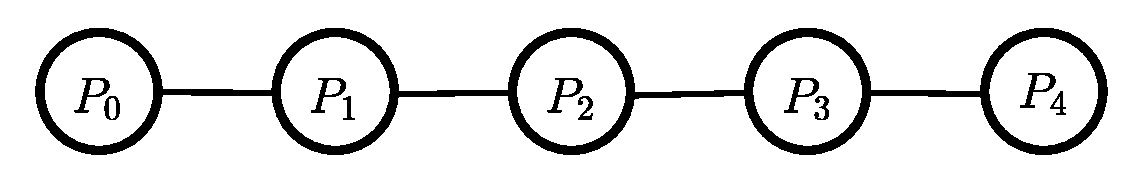
\includegraphics[width=9.5cm]{images/mesh1d}
\caption{Sieć jednowymiarowa}
\label{fig:model_mesh1d}
\end{figure}
Model składa się z \(p\) węzłów \(P_1, P_2, \dots, P_p\) połączonych ze sobą w ciąg, tj. węzeł \(P_i\) połączony jest z węzłem \(P_{i-1}\) i \(P_{i+1}\), o ile takie istnieją. Średnica takiej sieci wynosi \(p-1\), jej maksymalny stopień wynosi \(2\).\\
\end{przyklad}

\begin{przyklad}[Torus]
Siecią w topologii torusa nazywamy sieć liniowa z połączonymi końcami (rys. \ref{fig:model_torus1d}).
\begin{figure}[h]
\centering
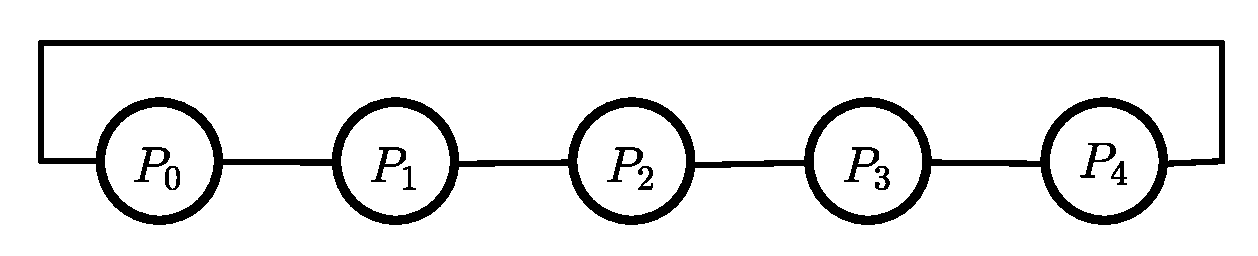
\includegraphics[width=10.5cm]{images/torus1d}
\caption{Torus jednowymiarowy}
\label{fig:model_torus1d}
\end{figure}

\end{przyklad}

\begin{przyklad}[Sieć dwuwymiarowa]
Dwuwymiarowa sieć jest dwuwymiarową wersją sieci liniowej. Składa się ona z \(p=m^2\) procesorów ułożonych w siatkę \(m\times m\) taką, że procesor \(P_{i,j}\) jest połączony z procesorem \(P_{i\pm 1, j}\) i \(P_{i, j\pm 1}\).\\
Średnica takiej sieci złożonej z \(p=m^2\) procesorów wynos \(\sqrt{p}\) a jej maksymalny stopień \(4\)
\begin{figure}[h]
\centering
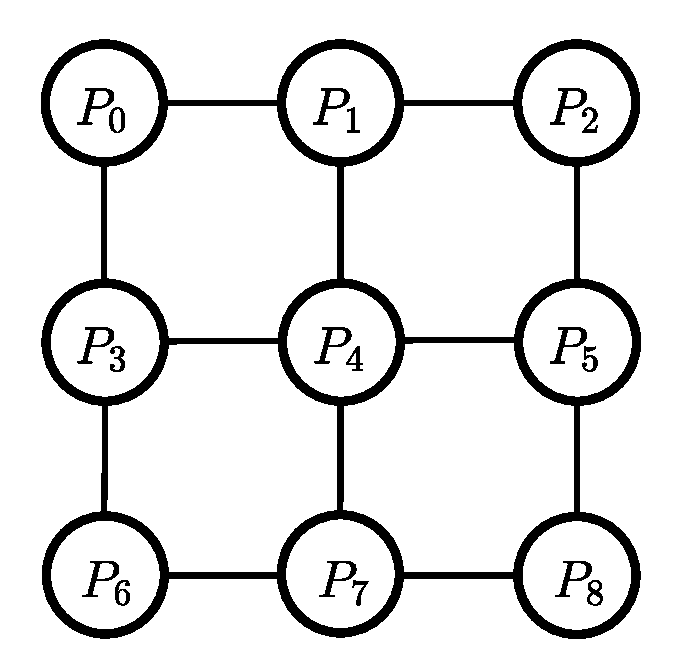
\includegraphics[width=5.5cm]{images/mesh2d}
\caption{Sieć dwuwymiarowa}
\label{fig:model_mesh2d}
\end{figure}
\end{przyklad}

\begin{przyklad}[Dwuwymiarowy torus]
Składa się ona z \(p=m^2\) procesorów ułożonych w siatkę \(m\times m\) (rys. \ref{fig:model_torus2d}) taką, że procesor \(P_{i,j}\) jest połączony z procesorem \(P_{i+1, j}\) i \(P_{i, j\pm 1}\).\\
Średnica takiej sieci złożonej z \(p=m^2\) procesorów wynos \(\sqrt{p}\) a jej maksymalny stopień \(4\)
\begin{figure}[h]
\centering
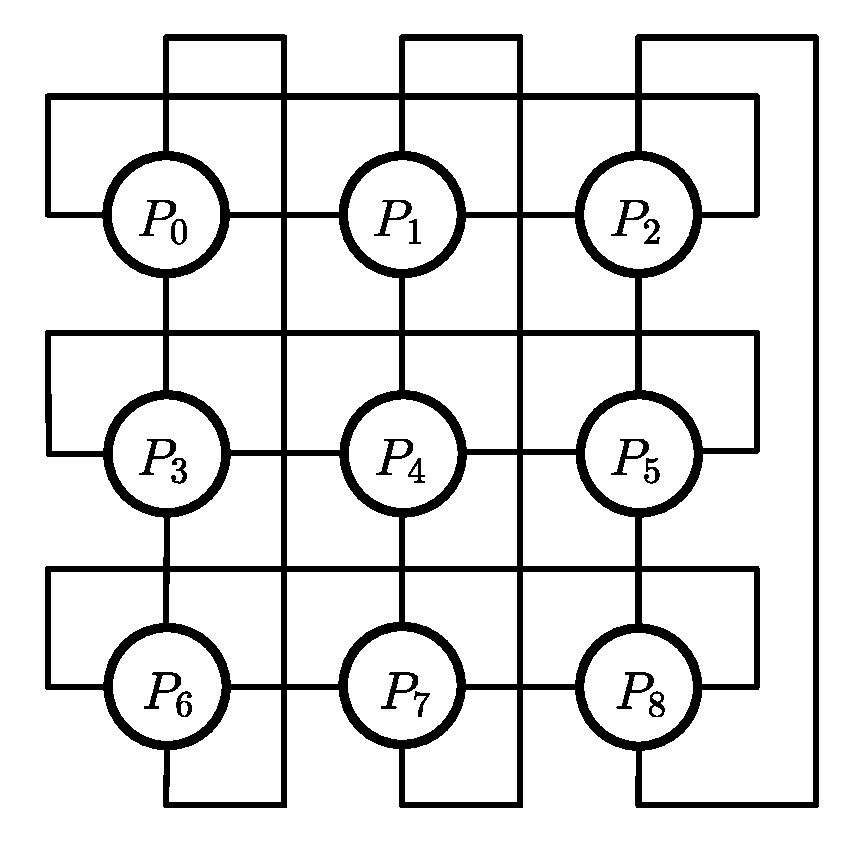
\includegraphics[width=7cm]{images/torus2d}
\caption{Torus dwuwymiarowy \(3\times3\)}
\label{fig:model_torus2d}
\end{figure}
\end{przyklad}


\begin{definicja}[Kostka Boola]
Niech \(i_{d-1}i_{d-2}\dots i_{0}\), gdzie \(0\leq i \leq p-1\) będzie binarną reprezentacją \(i\). Wówczas węzeł \({i}\) jest połaczony z węzłem \(P_{i^(j)}\), gdzie \(i^{(j)}=i_{d-1}\dots \overline{i_j} \dots i_0\) i \(\overline{i_j} = 1 - i_j\). Innymi słowy, dwa węzły są ze sobą połączone wtedy i tylko wtedy, gdy ich wskaźniki różnią się tylko jednym bitem.\\
\end{definicja}

\begin{przyklad}[Sieć hipersześcienna]
Sieć w topologii hipersześcianu skłąda się z \(p=2^d\) węzłów połączonych w d-wymiarową kostkę Boola.\\

Hipersześcian ma strukurę rekursywną. Kostkę \(d\)-wymiarową możemy rozszerzyć do \(d+1\) wymiarów przez połączenie poszczególnych węzłów do \(d\)-wymiarowych kostek.\\

Średnica d-wymiarowego hipersześcianu wynosi \(d=\log{p}\). Jest tak ponieważ odległośc w grafie między dwoma węzłami \(P_i\) i \(P_j\) jest równa liczbie pozycji bitów, którymi wskaźniki \(i\) i \(j\) różnią się między sobą. Stąd jest ona mniejsza lub równa \(d\), a ponadto odległość między \(P_0\) a \(P_{2^d-1}\) wynosi d. Każdy węzeł jest stopnia \(d=\log{p}\).
\end{przyklad}	
\begin{figure}[h]
\centering
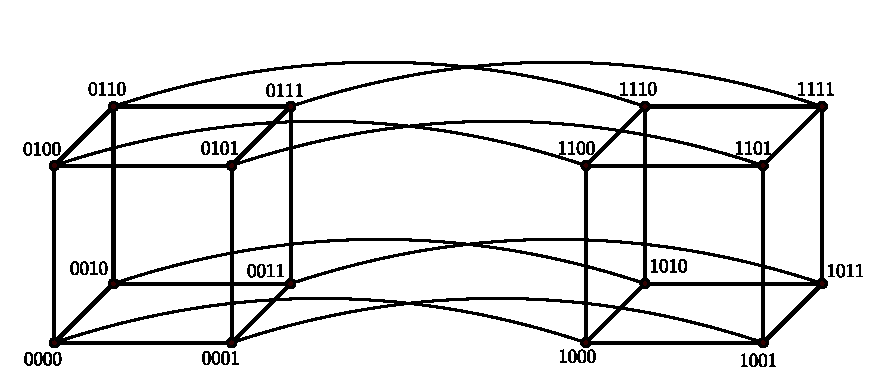
\includegraphics[width=32em]{images/systolic.eps}
\caption{Sieć w topologii hipersześcianu}
\label{fig:systolic}
\end{figure}
